\section{Performance Benchmark\label{sec:topologies.benchmark}}


In this section, we present some preliminary results regarding the performance of \thecontrib, as well as the influence of some constraints on performance.
Note that these results are based on a prototype implementation, and are more indicative of the potential of the approach than of its actual performance.
To evaluate our prototype, build a synthetic library $L$ of 253 unique sub-topologies with various characteristics, and perform a series of experiments to evaluate the performance of \thecontrib in various conditions.
We review the influence of the size of the library (\ie, $\#L$), the maximum number of nodes, the tree depth, and the number of service constraints on the performance of \thecontrib.
To this end, we measure the total derivation time (\ie, selection and composition), the number of generated sub-topology sets, and the number of generated final topologies (\ie, tree compositions of the sub-topology sets).


\subsection{Influence of the library size\label{sec:topologies.benchmark.library}}

\begin{tablefig}
  \centering
  \begin{minipage}[b]{0.45\textwidth}
    \begin{table}[H]
      \centering
      \small
      \begin{tabular}{l >{\ttfamily}l}
        \toprule
        \textbf{Parameter} & \normalfont\textbf{Value} \\
        \midrule
        Min. number of nodes & 10 \\
        Max. number of nodes & 25 \\
        Min. number of sub-topologies & 2 \\
        Max. number of sub-topologies & 6 \\
        Services list & empty \\
        Attacks list & empty \\
        Tree depth & 2 \\
        \bottomrule
      \end{tabular}
      \vspace{2ex}
      \caption{
        Fixed parameters for the library size benchmark.
        \label{tab:topologies.benchmark.library_size}
      }
    \end{table}
  \end{minipage}
  \hfill
  \begin{minipage}[b]{0.49\textwidth}
    \begin{figure}[H]
      \centering
      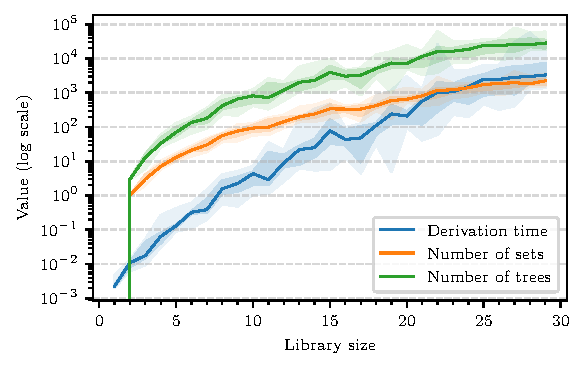
\includegraphics[width=\linewidth]{figures/library_size.pdf}
      \caption{
        Influence of the library size on the performance of \thecontrib.
        \label{fig:topologies.benchmark.library_size}
      }
    \end{figure}
  \end{minipage}
\end{tablefig}

The size of the library of sub-topologies has a direct on the number of combinations to explore.
To evaluate the influence of the library size on the performance of \thecontrib, we vary the library size $l$ from 1 to 29, with the other parameters fixed as in \Cref{tab:topologies.benchmark.library_size}.
For each run, build a smaller library $L'$ such as $L' \subset L$, and $\#L' = l$.
We randomly select $l$ sub-topologies from the full library to constitute the library set.
For each value of the library size, we perform ten experiments to increase the robustness of the results.

\Cref{fig:topologies.benchmark.library_size} displays the different metrics on a log scale.
We notably observe that the execution time increases exponentially with the library size.
This is expected due to the nature of the constraint solver and the tree composition algorithm.
The number of sub-topology sets and tree compositions also increase with the library size, but with a lower slope.
Note that even with a tree depth of 2, the number of tree compositions is superior to the number of sub-topology sets by a factor of 10.
Indeed, there is a combinatorial explosion of the number of possible compositions.


\subsection{Influence of the maximum number of nodes\label{subsec:topologies.benchmark.nodes}}

\begin{tablefig}
  \centering
  \begin{minipage}[b]{0.45\textwidth}
    \begin{table}[H]
      \centering
      \small
      \begin{tabular}{l >{\ttfamily}l}
        \toprule
        \textbf{Parameter} & \normalfont\textbf{Value} \\
        \midrule
        Min. number of nodes & 1 \\
        Min. number of sub-topologies & 1 \\
        Max. number of sub-topologies & 6 \\
        Services list & empty \\
        Attacks list & empty \\
        Tree depth & 2 \\
        Library size & 40 \\
        \bottomrule
      \end{tabular}
      \vspace{2ex}
      \caption{
        Fixed parameters for the maximum number of nodes benchmark.
        \label{tab:topologies.benchmark.nodes}
      }
    \end{table}
  \end{minipage}
  \hfill
  \begin{minipage}[b]{0.49\textwidth}
    \begin{figure}[H]
      \centering
      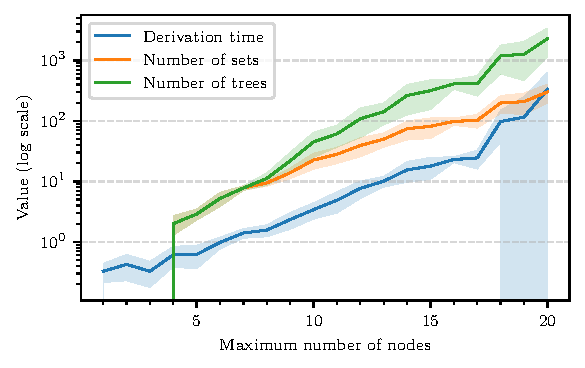
\includegraphics[width=\linewidth]{figures/max_nodes.pdf}
      \caption{
        Influence of the maximum number of nodes on the performance of \thecontrib.
        \label{fig:topologies.benchmark.nodes}
      }
    \end{figure}
  \end{minipage}
\end{tablefig}

We then evaluate the influence of the maximum number of nodes on the performance of \thecontrib.
We vary the maximum number of nodes from 1 to 20, with the other parameters fixed as in \Cref{tab:topologies.benchmark.nodes}.
For each value of the maximum number of nodes, we likewise perform ten experiments.

\Cref{fig:topologies.benchmark.nodes} displays the different metrics on a log scale.
Again, all metrics increase exponentially with the maximum number of nodes.
Indeed, this parameter indirectly influences the cardinality of the sub-topology sets generated, and thus the number of tree compositions.
Since we kept a tree depth of 2, the number of tree compositions is still significantly higher than the number of sub-topology sets.
Note that for a number of nodes inferior to 4, there are no solutions, are the topologies in our test library have at least 4 nodes.


\subsection{Influence of the tree depth\label{subsec:topologies.benchmark.depth}}

\begin{tablefig}
  \centering
  \begin{minipage}[b]{0.45\textwidth}
    \begin{table}[H]
      \centering
      \small
      \begin{tabular}{l >{\ttfamily}l}
        \toprule
        \textbf{Parameter} & \normalfont\textbf{Value} \\
        \midrule
        Min. number of nodes & 10 \\
        Max. number of nodes & 30 \\
        Min. number of sub-topologies & 2 \\
        Max. number of sub-topologies & 10 \\
        Services list & empty \\
        Attacks list & empty \\
        Library size & 20 \\
        \bottomrule
      \end{tabular}
      \vspace{2ex}
      \caption{
        Fixed parameters for the tree depth benchmark.
        \label{tab:topologies.benchmark.depth}
      }
    \end{table}
  \end{minipage}
  \hfill
  \begin{minipage}[b]{0.49\textwidth}
    \begin{figure}[H]
      \centering
      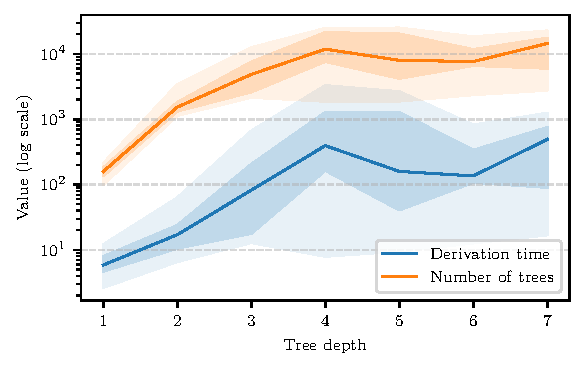
\includegraphics[width=\linewidth]{figures/tree_depth.pdf}
      \caption{
        Influence of the tree depth on the performance of \thecontrib.
        \label{fig:topologies.benchmark.depth}
      }
    \end{figure}
  \end{minipage}
\end{tablefig}

The next experiment evaluates the influence of the tree depth on \thecontrib's performance.
This parameter has no impact on the number of sub-topology sets, so we only measure the number of tree compositions and the execution time.
We vary the tree depth from 1 to 7, with the other parameters fixed as in \Cref{tab:topologies.benchmark.depth}.

\Cref{fig:topologies.benchmark.depth} displays the execution time and the number of tree compositions on a log scale.
Both increase exponentially with the tree depth, as expected, before reaching a plateau with a tree depth of 4.
This is due to the fact that the number of tree compositions is limited by the number of sub-topology sets, which in turn depends on the other constraints.
Consequently, the variations in the results are only due to the random sampling of the sub-topologies in the library.


\subsection{Influence of the number of service constraints\label{subsec:topologies.benchmark.services}}

\begin{table}
  \centering
  \caption{
    Fixed parameters for the number of service constraints benchmark.
    \label{tab:topologies.benchmark.services}
  }
  \small
  \begin{tabular}{l >{\ttfamily}l}
    \toprule
    \textbf{Parameter} & \normalfont\textbf{Value} \\
    \midrule
    Minimum number of nodes & 5 \\
    Maximum number of nodes & 15 \\
    Minimum number of sub-topologies & 2 \\
    Maximum number of sub-topologies & 6 \\
    Attacks list & empty \\
    Tree depth & 2 \\
    Library size & 40 \\
    \bottomrule
  \end{tabular}
\end{table}

This last experiment evaluates the influence of the number of service constraints on performance.
The library of sub-topologies is generated with a fixed number of available services, namely: \texttt{ldap}, \texttt{dbms}, \texttt{cms}, \texttt{dns}, \texttt{mail}, \verb|syslog_server|, \texttt{web}, \texttt{ftp}, \texttt{proxy}, and \verb|cloud_storage|.
We vary the number of services constraints from 1 to 9, with the other parameters fixed as in \Cref{tab:topologies.benchmark.services}.

\Cref{fig:topologies.benchmark.services-time,fig:topologies.benchmark.services-numbers} display the execution time and the numbers of sets and tree generations, respectively.
Unlike the other experiments, the execution time in almost constant here, due to the way these constraints are handled.
While the other constraints are implemented as exploration problems, the service and attack constraints are applied by pruning incompatible sub-topology sets.
Therefore, the number of sets and trees are progressively decreasing as the number of service constraints increases.
By the 6\textsuperscript{th} constraint, the resolution becomes infeasible, as there are no sub-topologies that satisfy all the constraints.
Increasing the maximum number of nodes and sub-topologies would allow for more solutions, but would also increase the execution time.


\begin{figure}
  \centering
  \begin{subfigure}[t]{0.49\linewidth}
    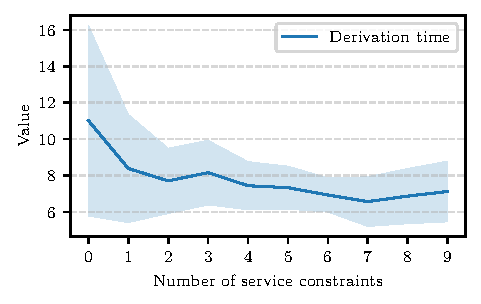
\includegraphics[width=\linewidth]{figures/services_time.pdf}
    \caption{
      Execution time.
      \label{fig:topologies.benchmark.services-time}
    }
  \end{subfigure}
  \hfill
  \begin{subfigure}[t]{0.49\linewidth}
    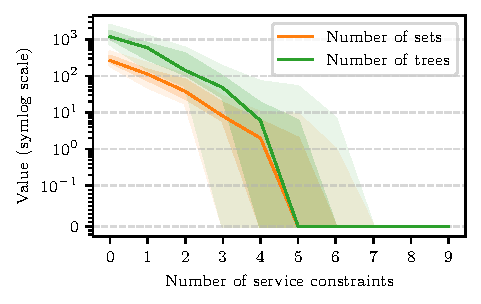
\includegraphics[width=\linewidth]{figures/services_numbers.pdf}
    \caption{
      Number of generated sets and tree compositions.
      \label{fig:topologies.benchmark.services-numbers}
    }
  \end{subfigure}
  \caption{
    Influence of the number of service constraints on the performance of \thecontrib.
    \label{fig:topologies.benchmark.services}
  }
\end{figure}